\section{How to login to midway}

\subsection{ssh}
\begin{frame}[fragile]
  \frametitle{Login to midway: ssh}
  \begin{itemize}
  \item {\color{mycolorcli}ssh} - {\color{mycolordef}s}ecure {\color{mycolordef}sh}ell. 
  \item {\color{mycolordef}If you have an account on midway}:
{\color{mycolorcli}
\begin{verbatim}
ssh -Y <userid>@midway2.rcc.uchicago.edu
\end{verbatim}
}
  \item The {\color{mycolorcli}\verb|-Y|} option allows to use not only command line interface (CLI) but also graphics (\verb|X-windows|) remotely - {\color{mycolordef}X-forwarding}
  \item This assumes that you have ssh client on your laptop.
  \item If you run Linux on your laptop, you have everything
  \item If you use Mac, than you should have ssh client although for X-forwarding you might need to install X11 server and client libraries, 
    which can be downloaded from the XQuartz project page: {\color{mycolorcli}\verb|https://www.xquartz.org|}
  \item If you have MS Windows, you might need to install a client: 
    for example {\color{mycolorcli}putty} or {\color{mycolorcli}bitvise} from  {\color{mycolorcli}\verb|http://www.putty.org|}. No X-forwarding.
  \item On Chromebook or any other OS you can use ssh extention to Chrome browser. No X-forwarding.
  \end{itemize}
\end{frame}

\subsection{yubikey}
\begin{frame}[fragile]
  \frametitle{Login to midway: yubikey}
  \begin{itemize}
  \item {\color{mycolordef}If you do not have an account on midway cluster}, use {\color{mycolordef}yubikey}:
    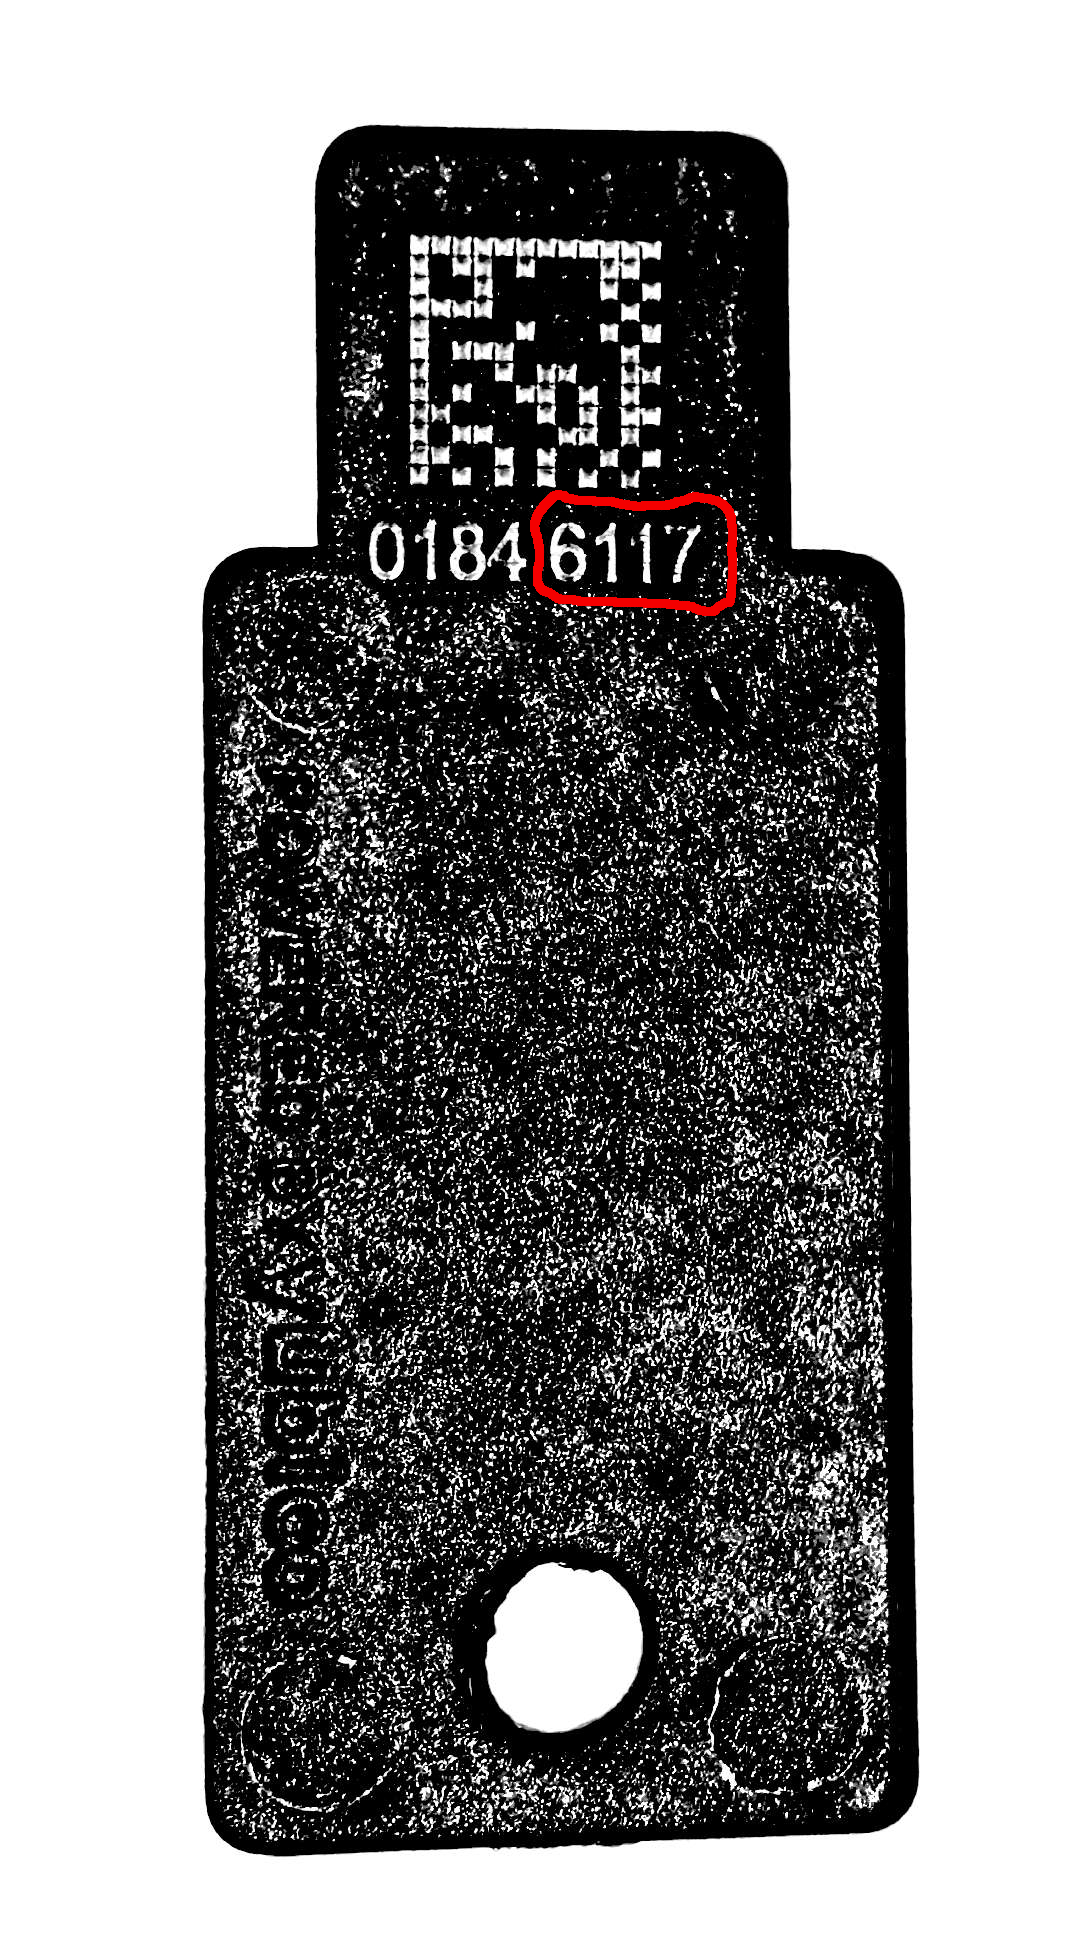
\includegraphics[width=1.5cm]{icons/yubikey1a.jpg}
    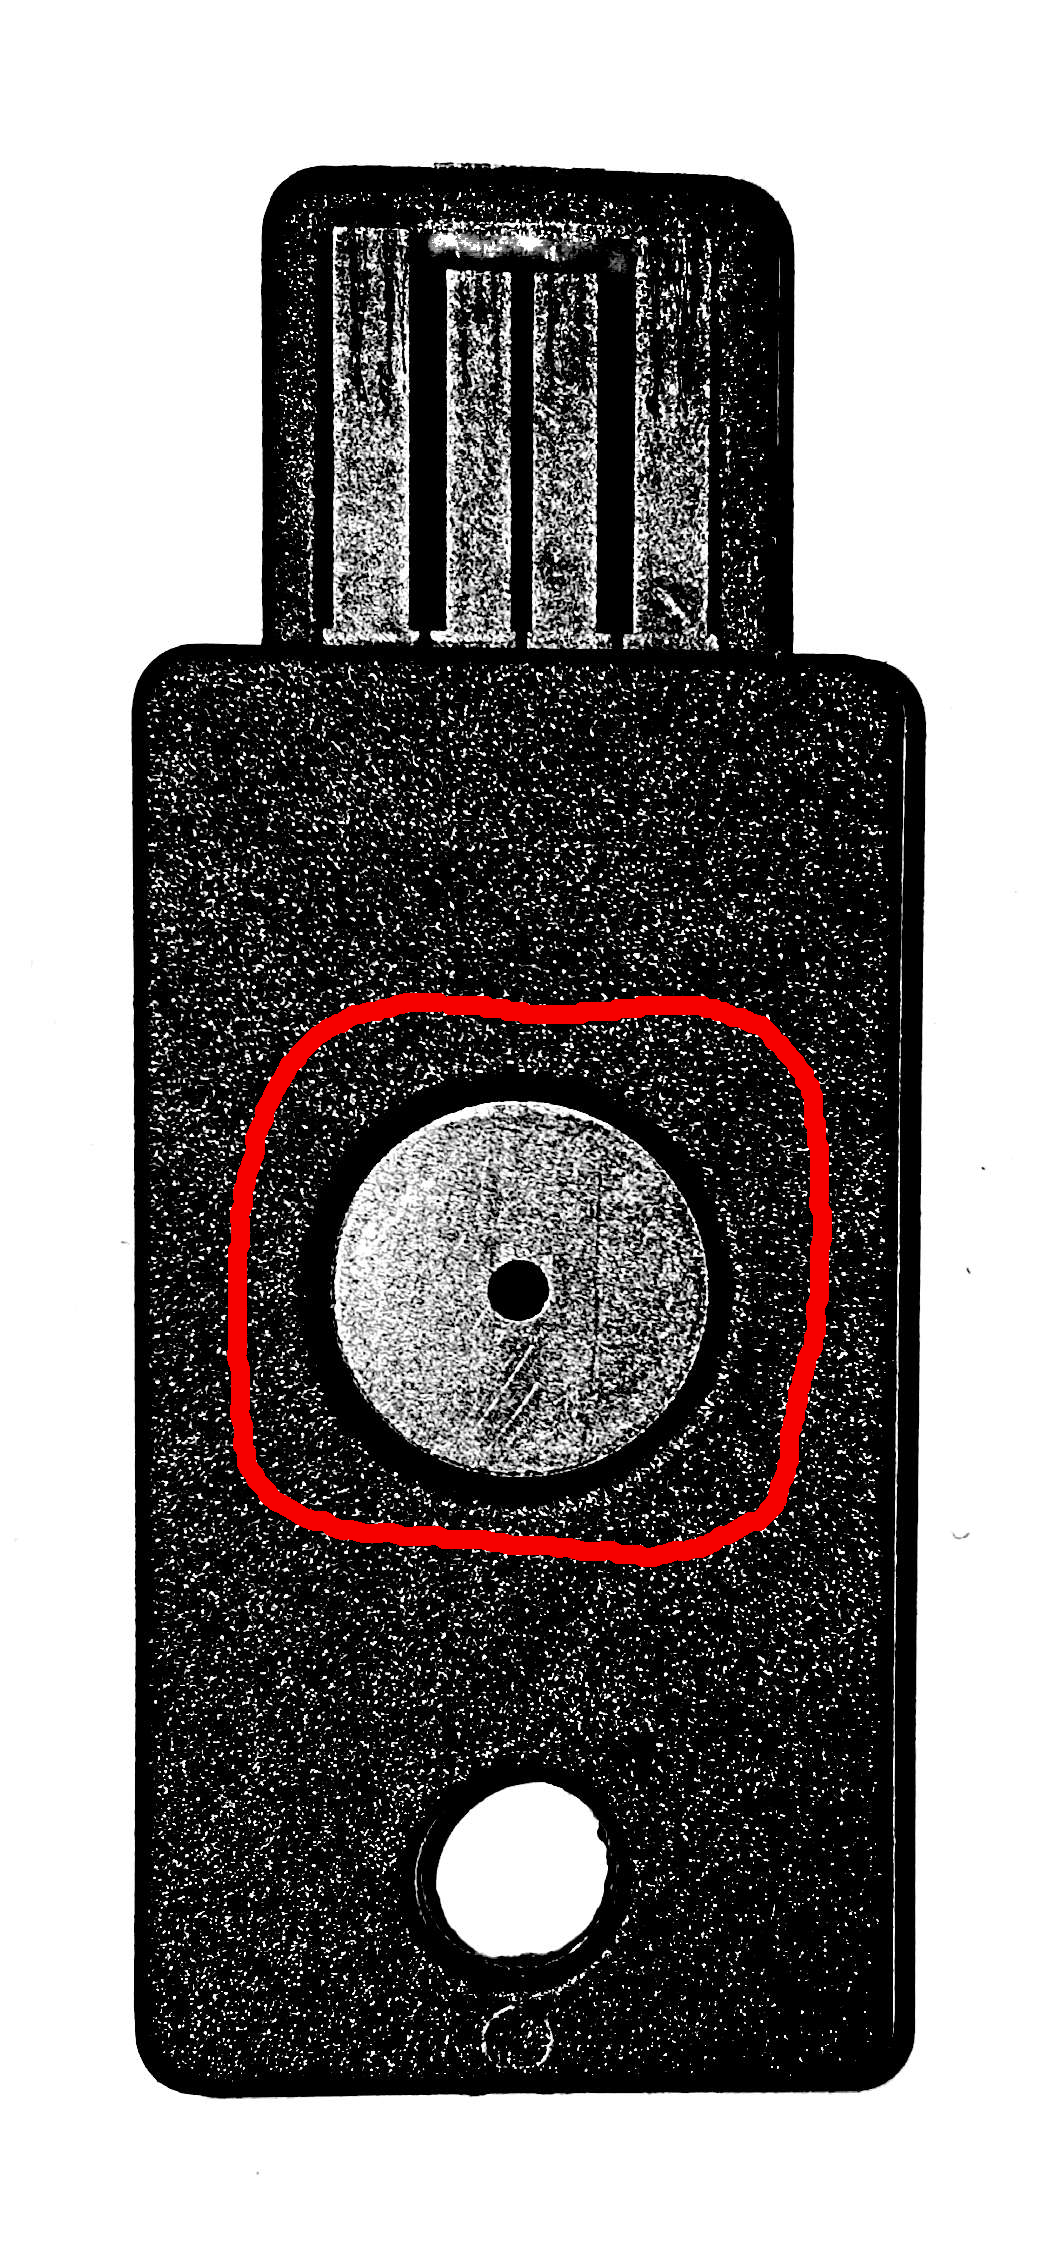
\includegraphics[width=1.3cm]{icons/yubikey2a.jpg}
    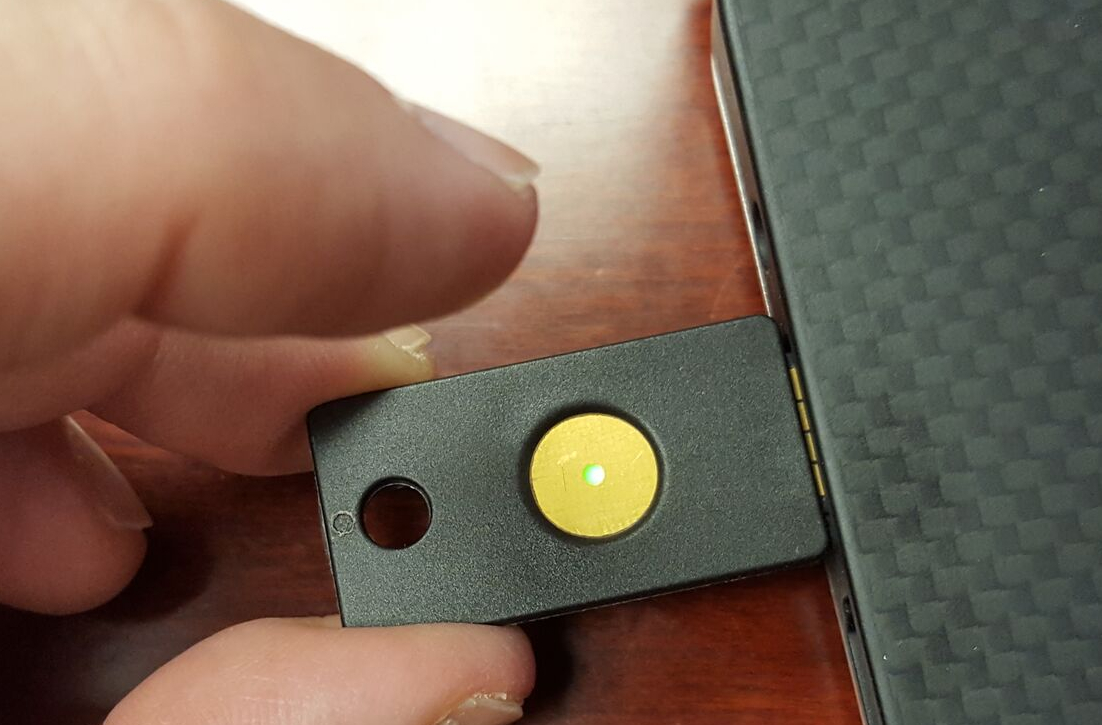
\includegraphics[width=3.3cm]{icons/yubikey3a.jpg}
  \item Use last 4 digits XXXX of yubikey as part of userid:
    {\color{mycolorcli}
\begin{verbatim}
ssh -Y rccguestXXXX@midway2.rcc.uchicago.edu
\end{verbatim}
    }
  \item Push the button when asked for password
  \end{itemize}
\end{frame}

\subsection{ThinLinc}
\begin{frame}[fragile]
  \frametitle{Login to midway: ThinLinc}
  \begin{itemize}
  \item ThinLinc should work with any OS on your laptop as long as you have a web browser. For many OSes you can also install client.
  \item ThinLinc server is a commercial product that might be running on some Linux sites but is not a standard part of Linux, contrary to ssh server, 
    and is not used in most other places. At RCC we run it on midway 1 \& 2 clusters but not on Hadoop cluster.
  \item {\color{mycolordef}ThinLinc does not work with yubikeys}.
  \end{itemize}
\end{frame}

\begin{frame}[fragile]
  \frametitle{Login to midway: ThinLinc}
  \begin{itemize}
    \item There are two ways to connect with ThinLinc to midway:
      \begin{itemize}
        \item Just use a web browser interface by pointing your browser to {\color{mycolorcli}\verb|https://midway2.rcc.uchicago.edu|}. 
          This might not work well for all browsers, you might have to try several: Chrome, Firefox, Safari...
        \item Install ThinLinc client from {\color{mycolorcli}\verb|https://www.cendio.com/thinlinc/download|}. 
          \begin{itemize}
          \item Configure the client to connect to {\color{mycolorcli}\verb|midway2.rcc.uchicago.edu|}
          \item You can specify the dimensions of the window in which it is running. I am usually using full screen.
          \item It does X-forwarding and you can use graphics, usually it works faster than vanilla ssh.
          \end{itemize}
      \end{itemize}
  \end{itemize}
\end{frame}
